\subsection{Area of expression decreases non-linearly}

The mean area of expression decreases in a non-linear way (an inverted saturation curve), with the major decrease occurring at very early development, from maternal to early gastrula stage (Fig. \ref{fig:Art-I-Area}).

This pattern of decrease is observed both in maternal genes (genes that are expressed from stage (1) and in zygotic genes (genes that start to be expressed later).
This highlight that a great proportion of the genes have already a restricted spatial pattern at early gastrulation, therefore the embryo is relatively well compartmentalized at this stage.

%Practically half of the genes in our set follow this decrease pattern: 46 of the genes (565 of 1218 genes) were characterized as having a non-linear decrease in their relative area (Appendix. S1). Our results are consistent with the hypothesis that the Drosophila embryo becomes compartmentalized in a progressively more fine-grained manner over developmental time. This is, most genes start being expressed in broad areas of the embryo and over time their expression becomes progressively restricted into smaller and smaller spatial domains.

\begin{figure}[h]
  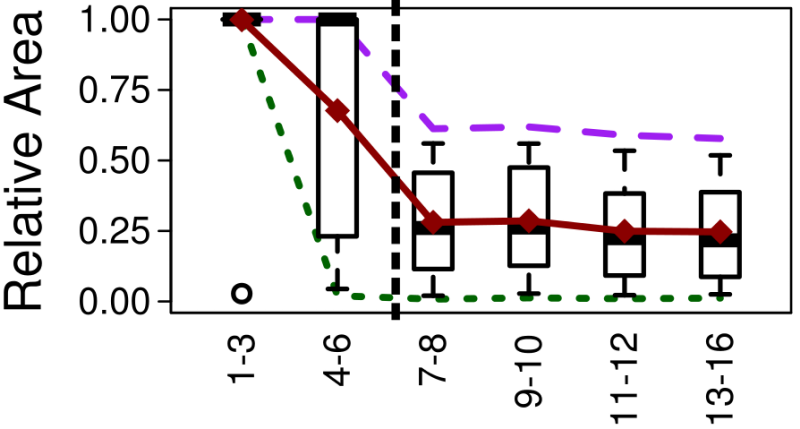
\includegraphics[width=0.4\textwidth]{./Images/Art-I/area.png}
  \centering
  \caption{Distribution plot of the relative area of expression for all genes in each stage. Diamonds represent the mean, boxes the IQR. Whiskers 10 and 90 percentiles. Dashed line represents the max values and dotted line the min values (mean of the last and first decile, respectively). Stages on the x-axis, vertical dashed line represents gastrulation entry.}
  \label{fig:Art-I-Area}
\end{figure}

%%%%%%%%%%%%%%%%%%%%%%%%%%%%%%%%%%%%%%%%%%%%%%%%%%%%%%%%%%%%%%%%%%%%%%%%%%%%%%%%%%%%% 

\subsection{TFs and GFs compartmentalize earlier}
The transcription factors (TFs;GO:0003700) and growth factor genes (GFs;GO:0008083) showed significantly smaller relative area of expression that the other genes in the blastoderm stage (Fig. \ref{fig:Art-I-TF-GF_area}).
	\nomenclature{GF}{Growth Factor}
	\nomenclature{KW}{Kruskal-Wallis test}
	
The TFs are expressed in significantly smaller areas than the rest of the genes in subsequent stages and the GFs are expressed in smaller areas at the blastoderm stage (stage 4-6) and the extended germ band stages (stage 9-10 and 11-12) (KW pvalue $<$ 0.05, Fig. \ref{fig:Art-I-TF-GF_area}).

 The fact that these genes have lower relative area (i.e., are more compartmentalized) than the rest of the genes, especially in the stage before entering gastrulation, is consistent with the leading role of these genes in driving pattern formation and the resulting compartmentalization of the embryo.
 
\begin{figure}[h]
  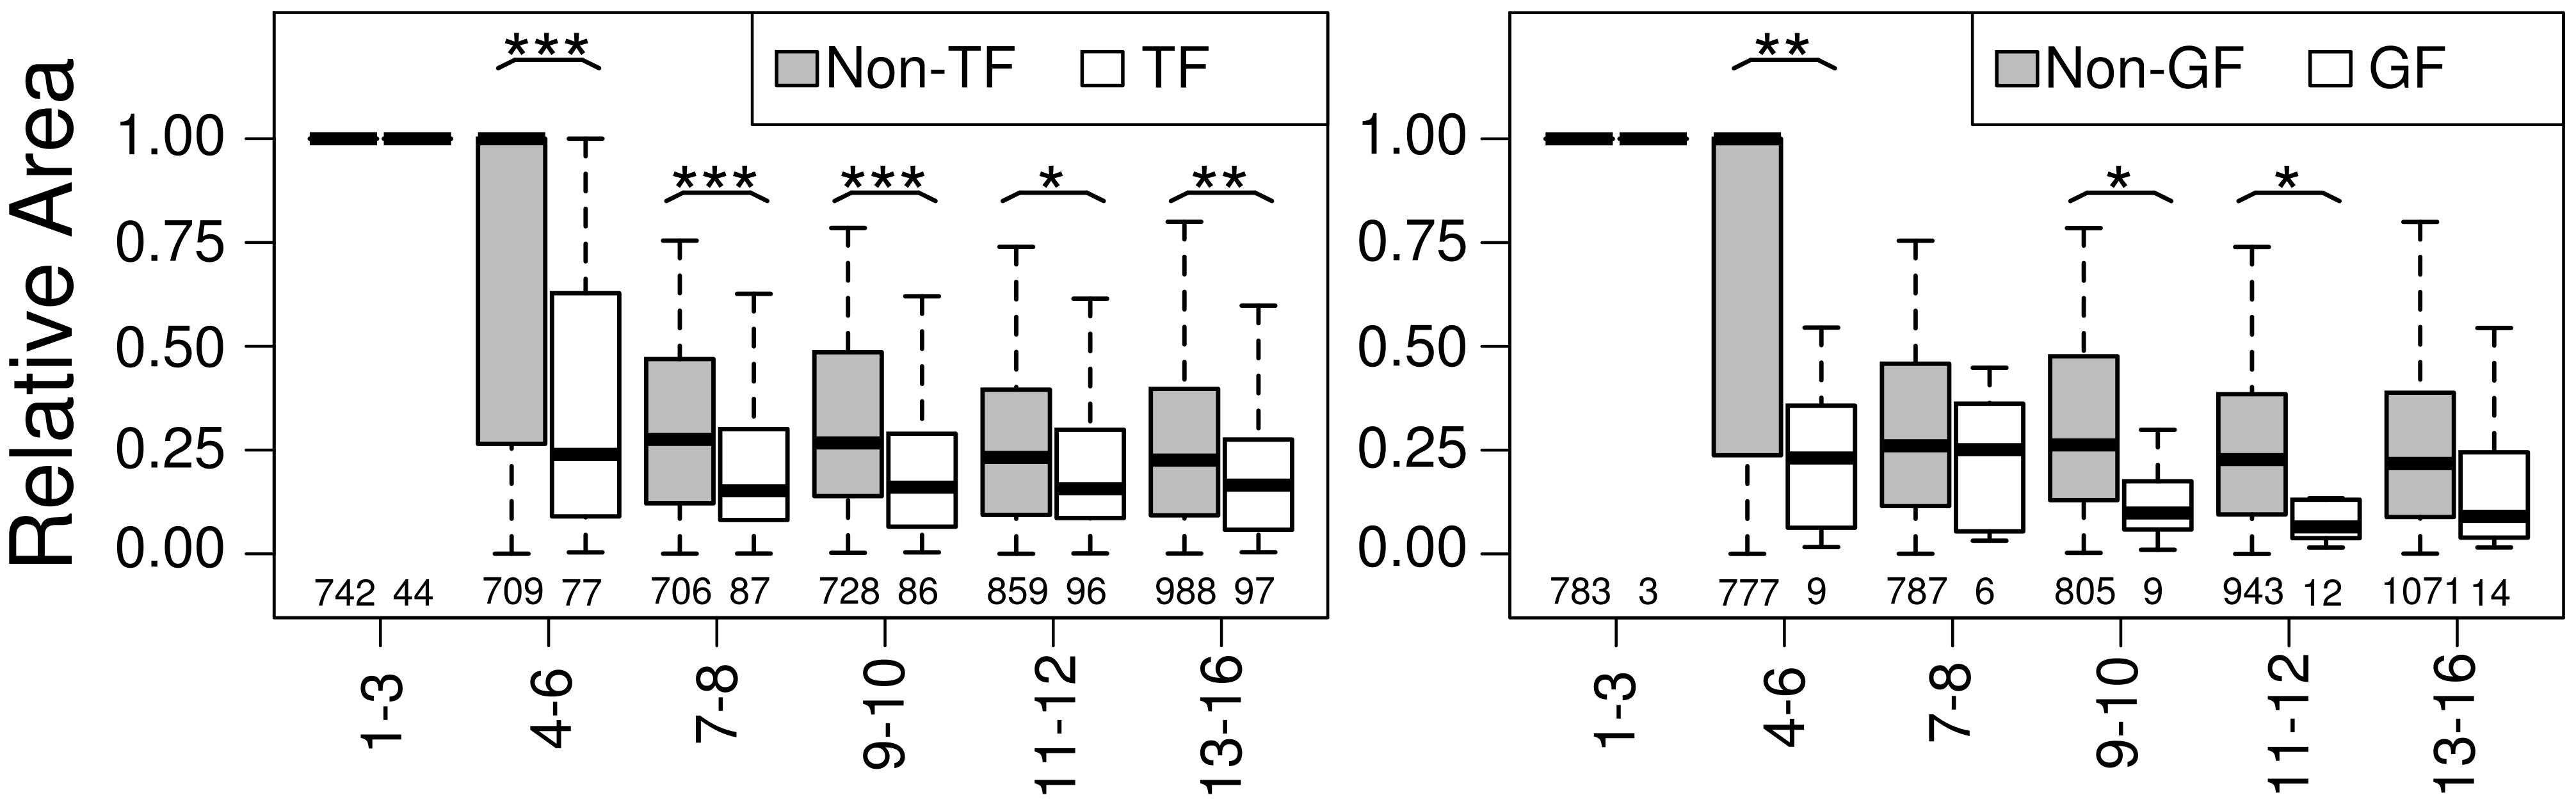
\includegraphics[width=0.8\textwidth]{./Images/Art-I/TF-GF_area.png}
  \centering
  \caption{Comparison between the relative area of expression of the transcription factors (white boxes) with the rest of the genes (gray boxes). On the right, same comparison for the growth factors (white boxes) and the rest of the genes (gray boxes). Stars represent significant values of p-values from Kruskal-Wallis test (*$<$0.05, **$<$0.01,***$<$0.001). Number of genes indicated below each box. }
  \label{fig:Art-I-TF-GF_area}
\end{figure}

%%%%%%%%%%%%%%%%%%%%%%%%%%%%%%%%%%%%%%%%%%%%%%%%%%%%%%%%%%%%%%%%%%%%%%%%%%%%%%%%%%%%% 
\subsection{Spatial disparity}

The disparity measure informs about how different genetically are the different regions of the embryo in different stages. This is complementary to the relative area of expression, as it could be that between two stages the relative area of expression decreases but not the disparity if the genes are expressed in the same part of the embryo.
Fig. \ref{fig:Art-I-disparity} shows that the disparity increases non-linearly following again a saturation curve, with the major change in the early stages.
In the blastoderm stage the disparity of the regions based only on the TFs is much greater than the one based on all the genes ((KW pvalue $<0.001$; Fig. \ref{fig:Art-I-disparity}) indicating that these genes account for a large portion of the diversity of gene expression patterns.

\begin{figure}[h]
  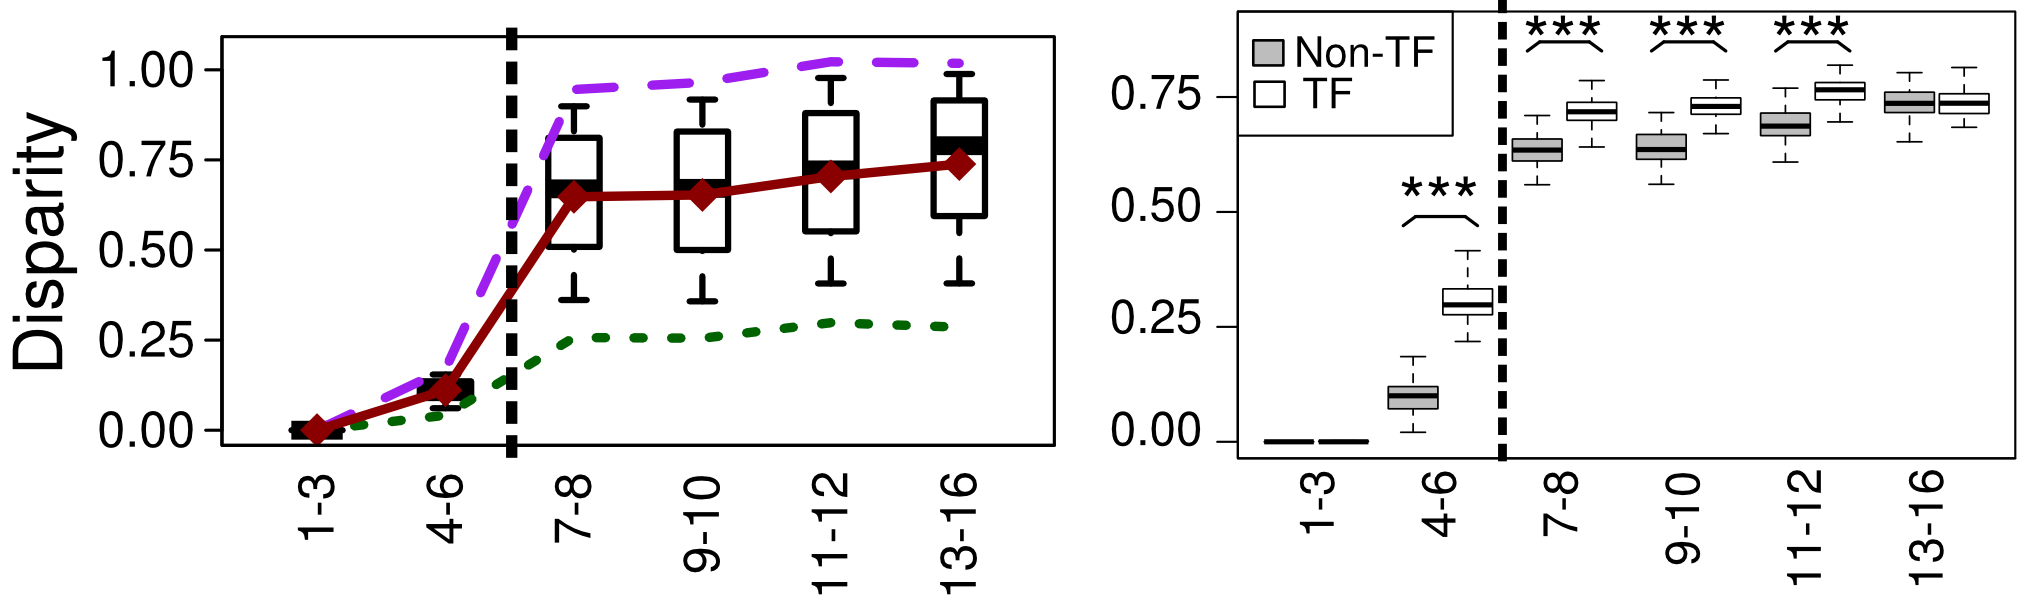
\includegraphics[width=0.8\textwidth]{./Images/Art-I/disparity.png}
  \centering
  \caption{Comparison between the relative area of expression of the transcription factors (white boxes) with the rest of the genes (gray boxes). On the right, same comparison for the growth factors (white boxes) and the rest of the genes (gray boxes). Stars represent significant values of p-values from Kruskal-Wallis test (*$<$0.05, **$<$0.01,***$<$0.001). Number of genes indicated below each box. }
  \label{fig:Art-I-disparity}
\end{figure}

